\section{Bremse 4.0}\label{sec:A_Bremse40}
Das vollständige Druckluftschema der \gls{Bremse 4.0}, bereits beschrieben in Kapitel \ref{sec:pKomp}, ist auf der nächsten Seite  zu sehen. Die Komponenten dazu lassen sich in Tabelle \ref{tab:Bremse40Komp} finden.
\begin{table}[h]
    \centering
    \begin{tabular}{|p{3em}cp{10.5em}p{18.5em}|}
    \hline
    Pos.  & \multicolumn{1}{p{2.5em}}{Anzahl} & Bezeichung & Zeichung / Kommentar  \\\hline
    02.01 & 2     & Aussenanzeige gls{HL} & Vergleichbar mit C-Druck-Anzeige \\
    02.02 & 2     & Endabsperrhahn 1,25" & z.B. Muffenkugelhahn Heco, Rückmeldekontakte \\
    
    04.01 & 1     & \gls{ep-Bremsen}n & Mg-Ventil NC \\
    04.02 & 1     & Kombinationsventil Bremse aus & Mechanisch gekuppelte Kugehähne, ein Antrieb, Rückmeldekontakte \\
    04.03 & 1     & Steuerventil & z.B SW4 mit G/P-Umstellung \\
    04.04 & 1     & Umstellantrieb G/P & Stellantrieb, Rückmeldekontakte \\
    04.05 & 1     & Vorsteuervenitl Schnelllösen & Mg-Ventil NC \\
    04.06 & 1     & Umstellventil Lastabbremsung & Kugelhahn 1/4", Rückmeldekontakte \\
    04.07 & 1     & Relaisventil & z.B. Faiveley VCAV \\
    04.08 & 2     & C-Druck-Sensor & 0-5 bar, 4...20 mA \\
    
    14.01 & 1     & Antrieb Feststellbremse & tbd, z.B. von PJM \\
    14.02 & 2     & Außenanzeige G/P & Mechanisch, Konstruktionsteil \\
    14.03 & 2     & Außenanzeige Leer/Beladen & Mechanisch, Konstruktionsteil \\
    14.04 & 2     & Außenanzeige Bremse aus & Mechanisch, Konstruktionsteil \\
    14.05 & 2     & Außenanzeige Feststellbremse & Mechanisch, Konstruktionsteil, 3 Zustände \\\hline
    \end{tabular}%
    \caption{Stückliste zum Druckluftschema der Bremse 4.0}
    \label{tab:Bremse40Komp}
\end{table}
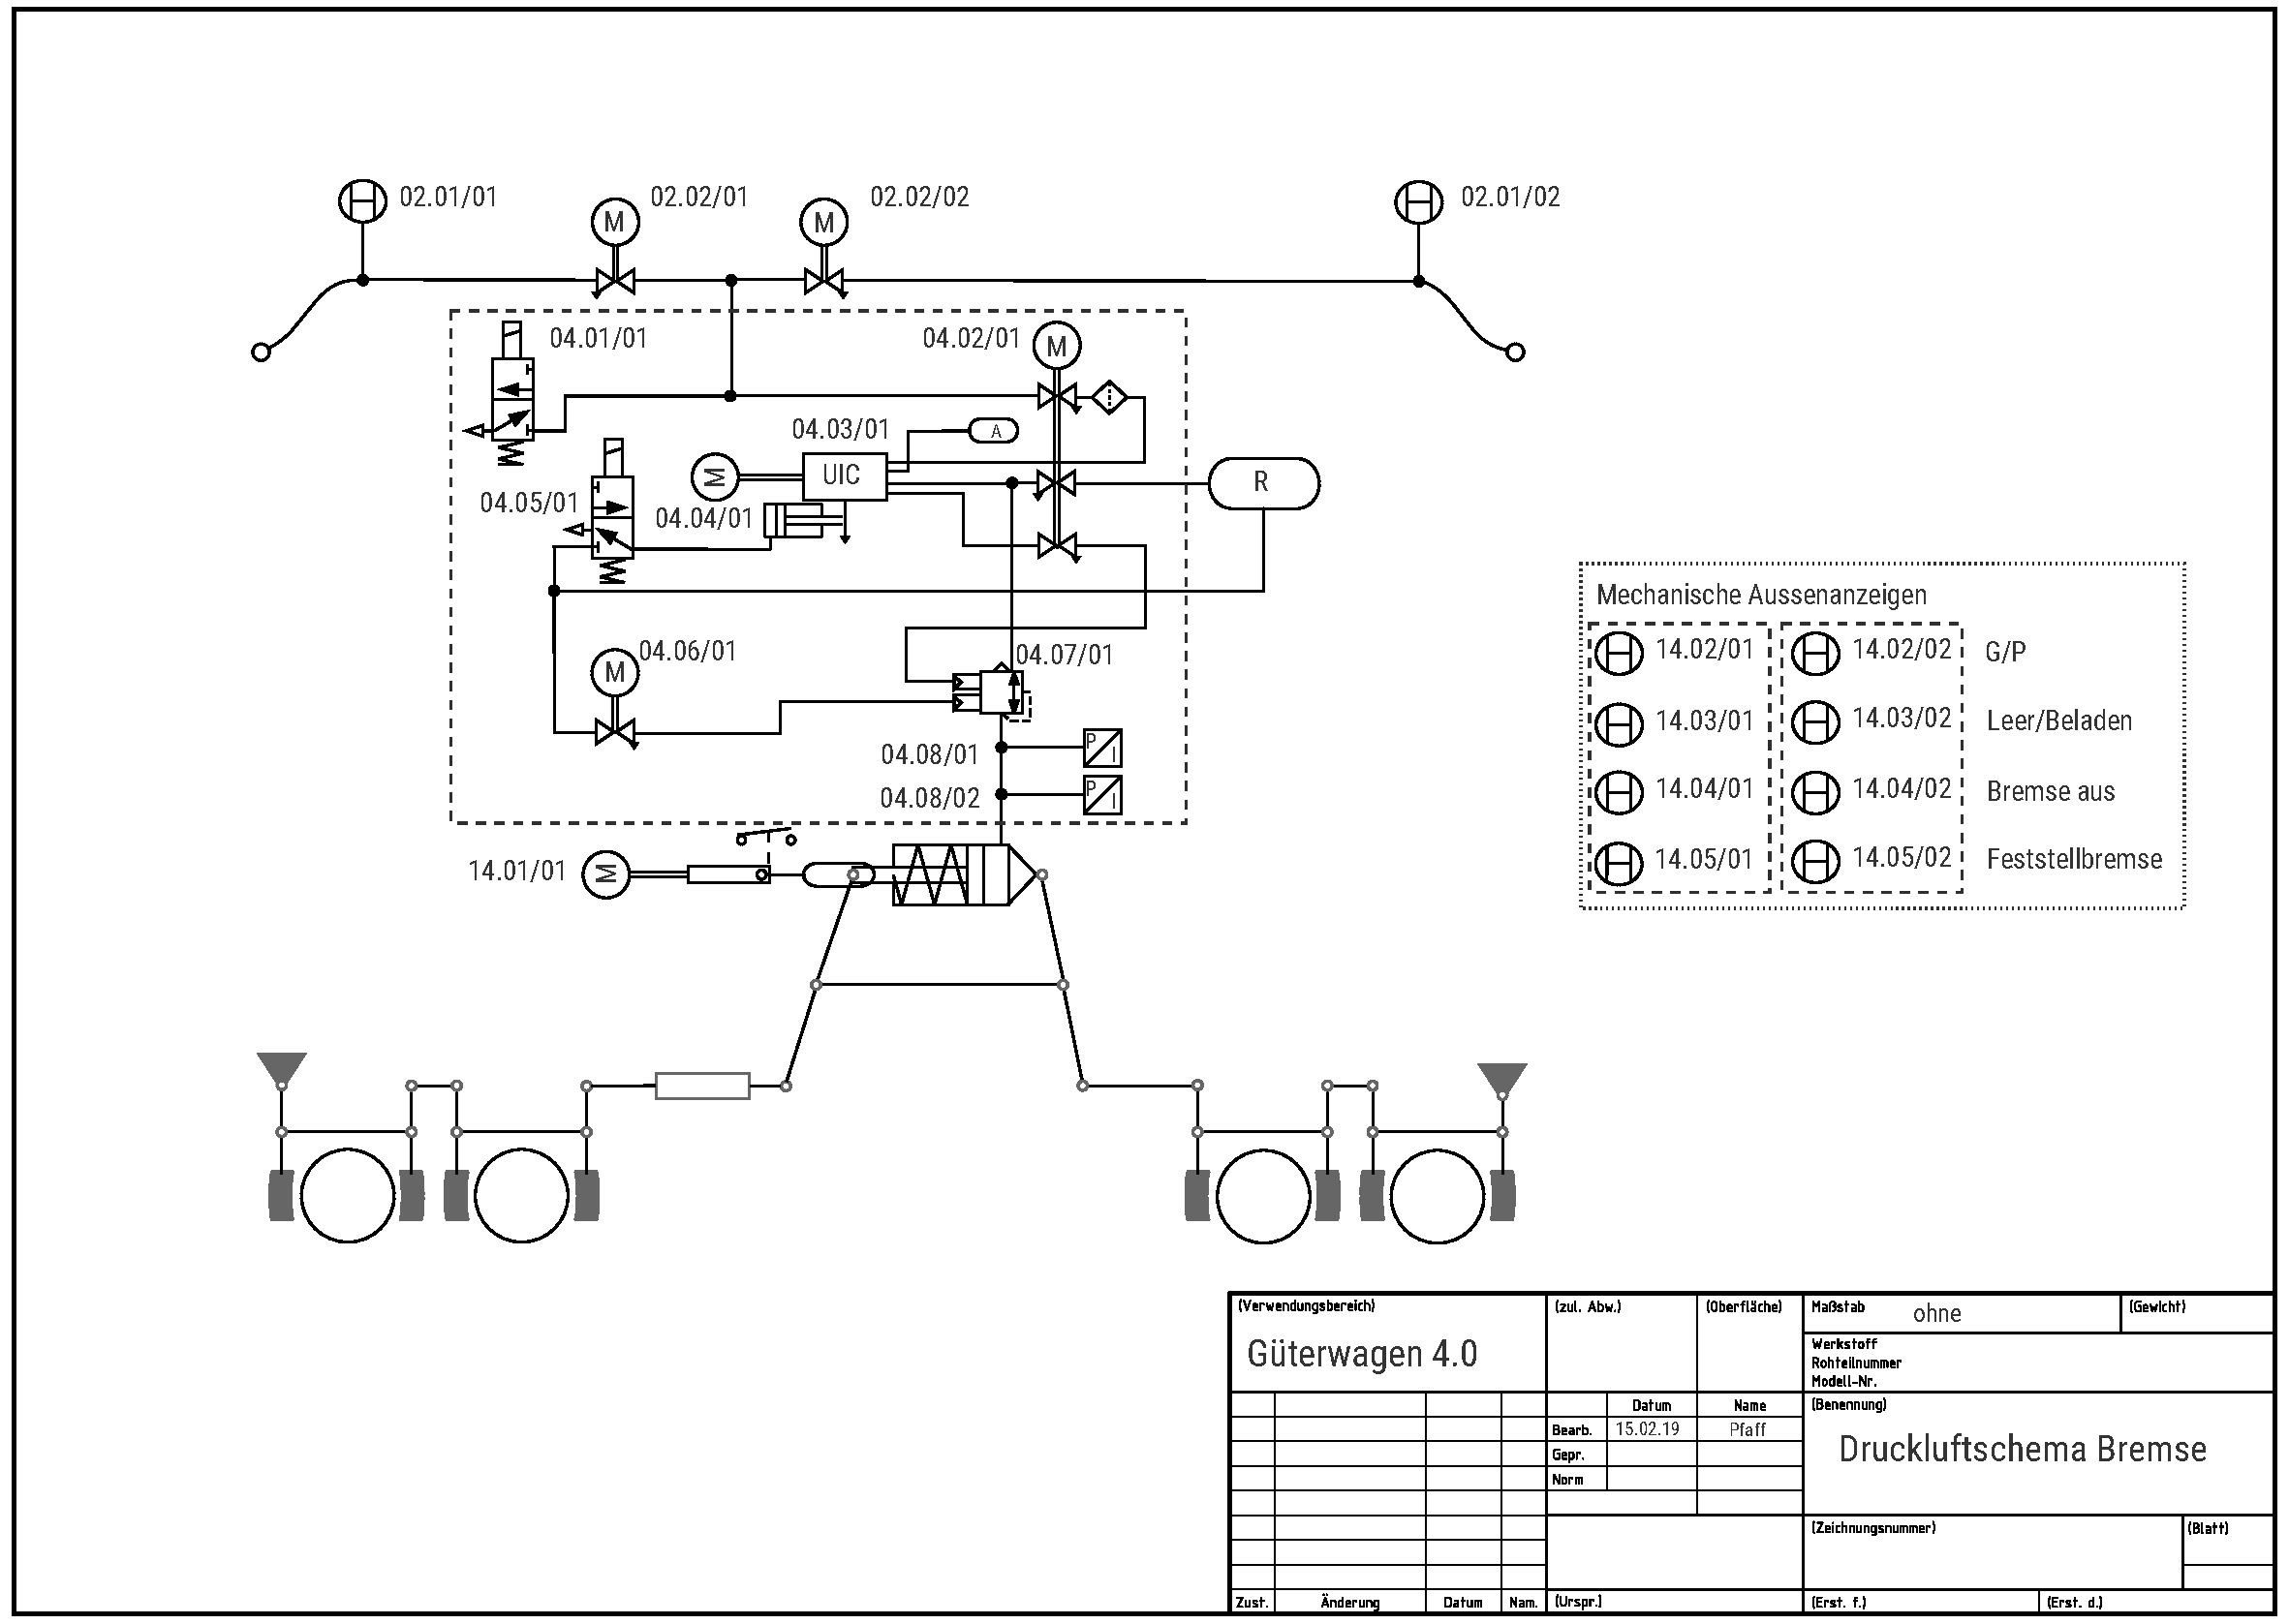
\includepdf[landscape=true, pages=-]{Bilder/PneumaticScheme.pdf}